\subsection{Lexikální analýza}
\label{subsec:lexer}
Úlohou Lexikálního analyzátoru je rozpoznávat jazykové lexémy a reprezentovat
je jako tokeny.

Lexikální analyzátor je implementací deterministického konečného
automatu. Jediný nedeterministický případ nastává tehdy, když má automat načítat znak ve tvatu $\backslash$ddd.
Případ je vyřešen implementací interního čítače počtu načtených číslic. Pokud čítač dosáhne hodnoty 3 a číslo je
v~intervalu $\langle 001 - 255\rangle$, je znak úspěšné načten, v~opačném případě je vygenerována chyba v lexikální
analýze.

Lexikální analyzátor je rozdělen do tří modulů: \ic|lexer.c|, \ic|lexer_fsm.c| a \ic|token.c|
. Modul \ic|token.c| obsahuje implementaci abstraktního datového typu token. Modul \ic|lexer_fsm.c|
obsahuje implementaci deterministického konečného automatu. Automat je oddělen od samožného lexeru z nutnosti simulování
přechodu z jedné konfigurace do konfigurace jiné v jednotkových testech. Modul \ic|lexer.c| poskytuje funkci
\ic|lexer_next_token|, která řídí činnost deterministického konečného automatu vrací další token. Chyba v lexikální
analýze je rozpoznána navrácením chybného tokenu.

\vspace*{16px}
\begin{figure}[htbp]
    \label{subsec:automat}
    \caption{Grafická reprezentace konečného automatu}
    \centering
    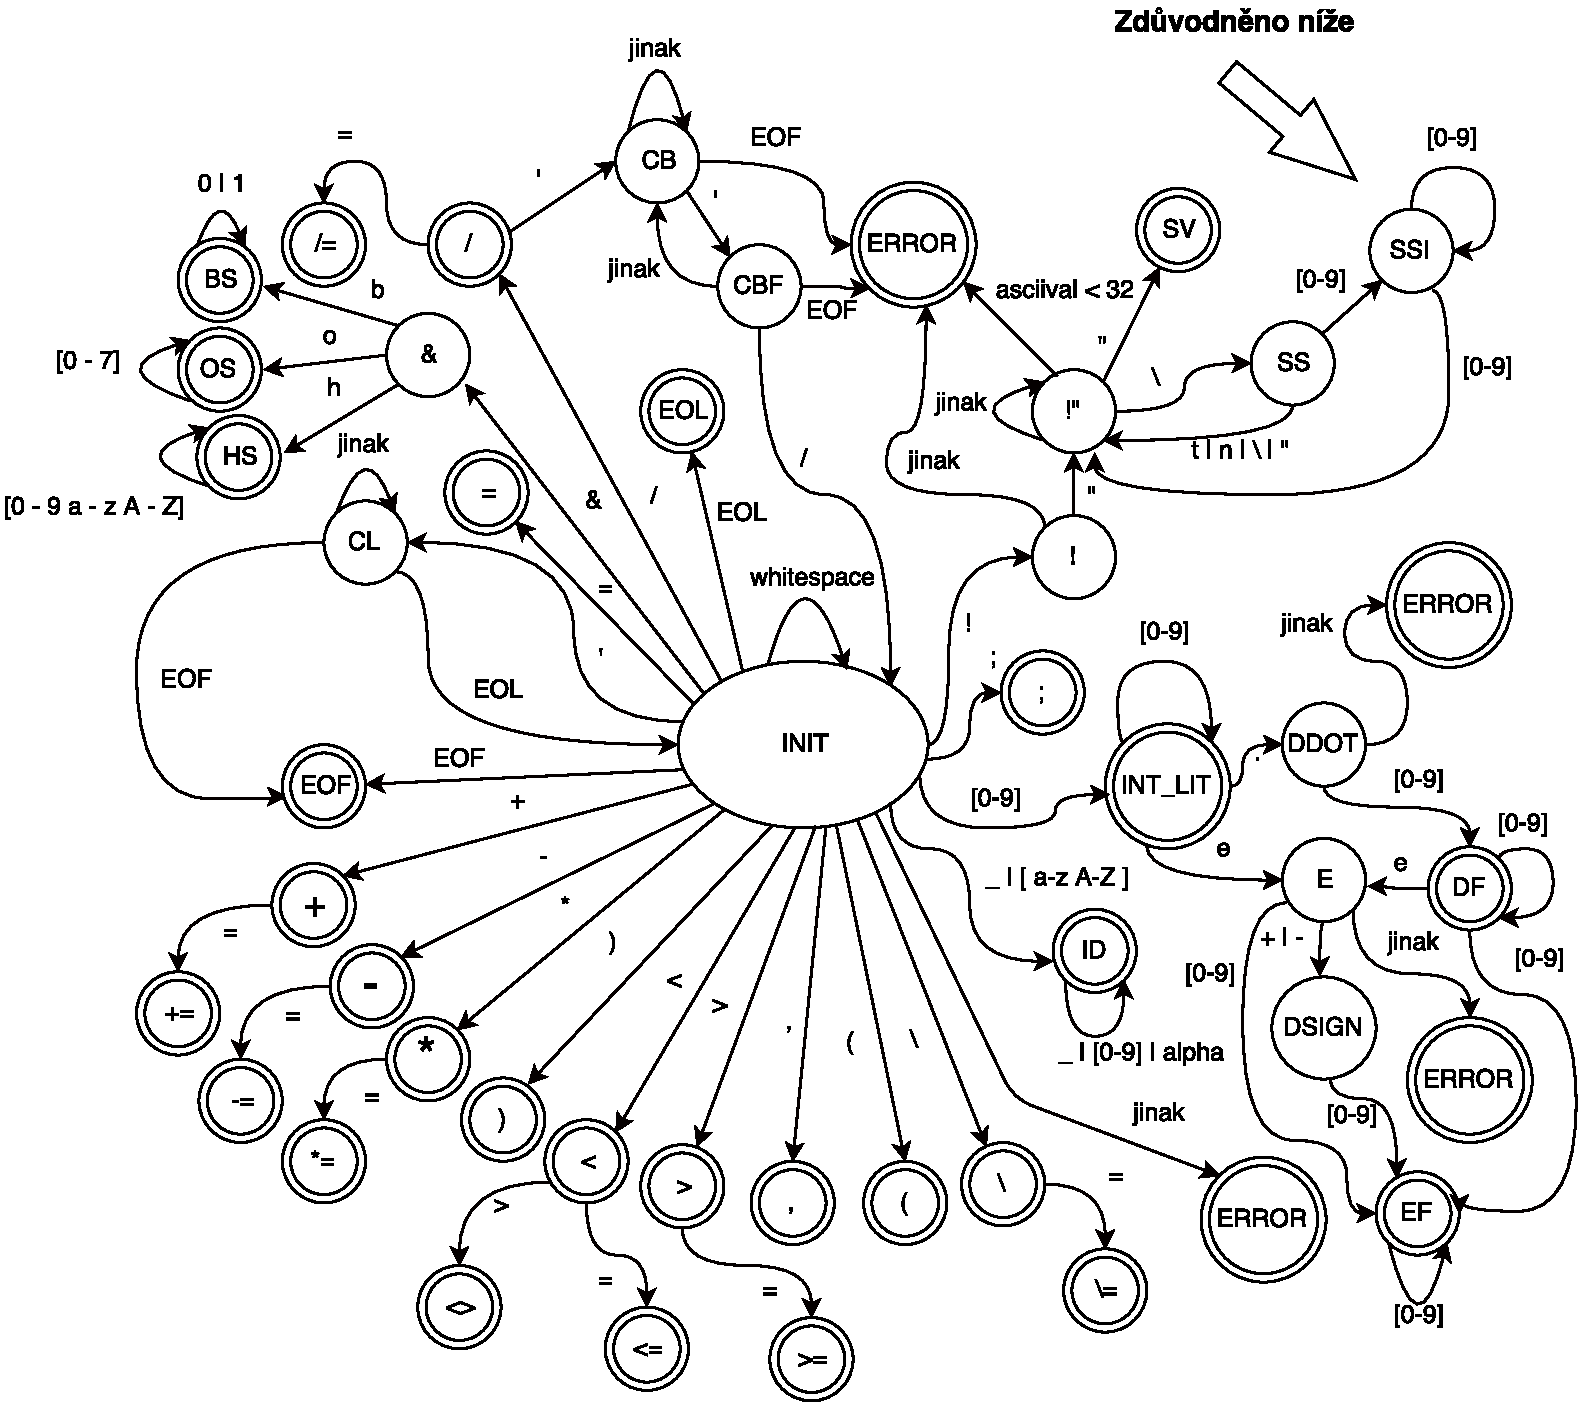
\includegraphics[width=1\textwidth, angle=0]{src/assets/automat.pdf}
\end{figure}


\subsection{Synataktická analýza}
Syntaxí řízený překlad je naimplementován v~modulu \ic|parser.c|, pro syntaktickou analýzu programu jako takového je
použita SA shoda dolů, konkrétně metoda rekurzivního sestupu. Pro každé pravidlo z~LL gramatiky existuje v~tomto
modulu funkce realizující toto pravidlo.

Pro snažší zápis v~jazyce C byl implementován poloautomatický systém generování těchto funkcí za pomocí maker.
Makra konkrétní pravidlo zavolají a zkontrolují jeho splnění. Pro kontrolu přítomnosti terminálu bylo
naimplemntováno makro \ic|CHECK_TOKEN(TOKEN_TYPE)|, pro zavolání pravidla bylo naimplementováno pravidlo
\ic|CALL_RULE(NAME_OF_RULE)|. Pro podmínečná volání pravidel makro
\ic|CHECK_RULE(token_type == TOKEN_TYPE, NAME_OF_RULE, REWIND_AND_SUCCESS)| - Při použití se zavolá pravidlo
\ic|NAME_OF_RULE| v~případě, že je následující token typu \ic|TOKEN_TYPE| a jestliže bylo úspěšné, další načtený
token navrátí zpět lexikálnímu analyzátoru a prohlásí volání za úspěšné.

Všechny pravidla pracují nad strukturou \ic|Parser|, která zapouzdřuje základní komponenty pro syntaxí řízený překlad.
Jedná se především od struktury \ic!ParserSemantic!, \ic!CodeConstructor! a \ic!Lexer!. První zmíněná zajištuje sémantické
kontroly programu; uchovává \emph{registr symbolů}, dočasné proměnné, pravidla pro implicitní konverze datových typů či
aktuální scénář SA. Konstruktor kódu je poté popsán v~příslušné sekci \ref{subsec:code-constructor}, Lexer v~sekci
\ref{subsec:lexer}.

Pro analýzu výrazů není analýza shora dolů příliš vhodná, proto byla
použita metoda zdola nahoru v~našem případě založená na precedenční
syntaktické analýza implementovaná v~souboru \ic|parser_expr.c|.

Na celý program je použita funkce \ic|parser_parse| z~modulu \ic|parser.c|. V~případě že je jako neterminál
očekáván výraz, je volána funkce \ic|parser_parse_expr| z~modulu \ic|parser_expr.c|, která provede precedenční
syntaktickou analýzu výrazu. Některé derivace neterninálu \ic|<statement_single>| nemohou v určitém kontextu nastat
Například příkaz \ic|return| se nemůže vyskytovat v~hlavním bloku. Kdybychom toto chtěli řešit
přímo pomocí gramatiky, bylo by to možné ale gramatika by narozstla do monstrózních rozměrů.
V tomto případě nám napomáhají sémantické akce.

Neterminál \ic|<eols>| slouží ke "zkonzumování" všech přebytečných znaků EOL. Jedná se o~univerzální neterminál použitelné
i mimo naší gramatiku, proto pro všechny terminály kromě \ic|EOL| používá poravidlo 60. Toto pravidlo je voláno kdykoliv
je v programu možný výskyt více prázdných řádků.

\subsubsection{Gramatika a LL tabulka}
\begin{normalsize}
    \begin{enumerate}
        {\small
        \item <prog> $\rightarrow$ <body> <eols> EOF
        \item <body> $\rightarrow$ <definitions\_block> <scope> <shared\_variables\_declarations>

        \item <definitions\_block> $\rightarrow$ <eols> <definitions>

        \item <definitions> $\rightarrow$ <definition> <definitions\_block>
        \item <definitions> $\rightarrow$ $\varepsilon$

        \item <definition> $\rightarrow$ <function\_declaration>
        \item <definition> $\rightarrow$ <function\_definition>
        \item <definition> $\rightarrow$ <shared\_variable\_declaration>

        \item <function\_definition> $\rightarrow$ <function\_header> EOL <eols> <statements> END FUNCTION EOL
        \item <function\_declaration> $\rightarrow$ DECLARE <function\_header> EOL

        \item <function\_header> $\rightarrow$ FUNCTION IDENTIFIER (<function\_params>) AS <type> EOL

        \item <function\_params> $\rightarrow$ $\varepsilon$
        \item <function\_params> $\rightarrow$ <function\_param> <function\_n\_param>

        \item <function\_n\_param> $\rightarrow$ $\varepsilon$
        \item <function\_n\_param> $\rightarrow$ , <function\_param> <function\_n\_param>

        \item <function\_param> $\rightarrow$ IDENTIFIER AS <type>


        \item <type> $\rightarrow$ INTEGER
        \item <type> $\rightarrow$ BOOLEAN
        \item <type> $\rightarrow$ STRING
        \item <type> $\rightarrow$ DOUBLE

        \item <statements> $\rightarrow$ $\varepsilon$
        \item <statements> $\rightarrow$ <statement\_single> EOL <eols> <statements>


        \item <statement\_single> $\rightarrow$ <identifier\_assignment>
        \item <statement\_single> $\rightarrow$ <input>
        \item <statement\_single> $\rightarrow$ <return>
        \item <statement\_single> $\rightarrow$ <print>
        \item <statement\_single> $\rightarrow$ <condition>
        \item <statement\_single> $\rightarrow$ <while\_>
        \item <statement\_single> $\rightarrow$ <variable\_declaration>
        \item <statement\_single> $\rightarrow$ <static\_variable\_declaration>
        \item <statement\_single> $\rightarrow$ <scope>

        \item <variable\_declaration> $\rightarrow$ DIM IDENTIFIER AS <type> <declaration\_assignment>
        \item <declaration\_assignment> $\rightarrow$ E
        \item <declaration\_assignment> $\rightarrow$ <assignment>

        \item <shared\_variables\_declarations> $\rightarrow$ E
        \item <shared\_variables\_declarations> $\rightarrow$ <shared\_variable\_declaration>
        \item <shared\_variable\_declaration> $\rightarrow$ DIM SHARED IDENTIFIER AS <type> <declaration\_assignment>

        \item <static\_variable\_declaration> $\rightarrow$ STATIC IDENTIFIER AS <type> <declaration\_assignment>

        \item <return> $\rightarrow$ RETURN <expr>

        \item <assignment> $\rightarrow$ = <expression>
        \item <assignment> $\rightarrow$ <modify> <expression>
        \item <modify> $\rightarrow$ +=
        \item <modify> $\rightarrow$ -=
        \item <modify> $\rightarrow$ *=
        \item <modify> $\rightarrow$ /=
        \item <modify> $\rightarrow$ $\backslash$=

        \item <print> $\rightarrow$ PRINT <print\_expression> <print\_expressions>
        \item <print\_expressions> $\rightarrow$ E
        \item <print\_expressions> $\rightarrow$ <print\_expression> <print\_expressions>
        \item <print\_expression> $\rightarrow$ <expression> SEMICOLON

        \item <while\_> $\rightarrow$ DO WHILE <expression> EOL <eols> <cycle\_statements> LOOP

        \item <input> $\rightarrow$ INPUT IDENTIFIER

        \item <identifier\_assignment> $\rightarrow$  IDENTIF <assignment>

        \item <condition> $\rightarrow$ IF <expr> THEN EOL <eols> <statements> <condition\_elseif> <condition\_else> END IF
        \item <condition\_elseif> $\rightarrow$ $\varepsilon$
        \item <condition\_elseif> $\rightarrow$ ELSEIF <expr> THEN EOL <eols> <statements> <condition\_elseif>

        \item <condition\_else> $\rightarrow$ $\varepsilon$
        \item <condition\_else> $\rightarrow$ ELSE EOL <eols> <statements>

        \item <eols> $\rightarrow$ $\varepsilon$
        \item <eols> $\rightarrow$ EOL <eols>
        }
        \newpage
        \begin{landscape}
            \begin{table}[htbp]
                \label{table:prec}
                \centering
                \caption{LL tabulka 1. část}
                \begin{tabular}{|l|l|l|l|l|l|l|l|l|l|l|l|l|l|l|l|l|l|l|l|l|l|l|l|l|}
                    \hline
                    & {\rotatebox[origin=c]{90}{Operátor}}  & ( & ) & {\rotatebox[origin=c]{90}{identifier}}
                    & {\rotatebox[origin=c]{90}{integer literal}} & = & ; & {\rotatebox[origin=c]{90}{as}}
                    & {\rotatebox[origin=c]{90}{asc}}

                    & {\rotatebox[origin=c]{90}{delcare}} & {\rotatebox[origin=c]{90}{dim}}
                    & {\rotatebox[origin=c]{90}{do}} & {\rotatebox[origin=c]{90}{double}}
                    & {\rotatebox[origin=c]{90}{else}} & {\rotatebox[origin=c]{90}{end}}
                    & {\rotatebox[origin=c]{90}{chr}} & {\rotatebox[origin=c]{90}{function}}

                    & {\rotatebox[origin=c]{90}{if}} & {\rotatebox[origin=c]{90}{input}}
                    & {\rotatebox[origin=c]{90}{integer}} & {\rotatebox[origin=c]{90}{length}}
                    & {\rotatebox[origin=c]{90}{loop}} & {\rotatebox[origin=c]{90}{print}}
                    & {\rotatebox[origin=c]{90}{return}}
                    \\ \hline

                    <prog>&&&&&&&&&&1&&&&&&&1&&&&&&&
                    \\ \hline
                    <body>&&&&&&&&&&2&&&&&&&2&&&&&&&
                    \\ \hline
                    <def\_b>&&&&&&&&&&3&&&&&&&3&&&&&&&
                    \\ \hline
                    <defs>&&&&&&&&&&4&&&&&&&4&&&&&&&
                    \\ \hline
                    <def>&&&&&&&&&&6&&&&&&&7&&&&&&&
                    \\ \hline
                    <f\_def>&&&&&&&&&&&&&&&&&9&&&&&&&
                    \\ \hline
                    <f\_he>&&&&&&&&&&&&&&&&&10&&&&&&&
                    \\ \hline
                    <f\_pas>&&&12&13&&&&&&&&&&&&&&&&&&&&
                    \\ \hline
                    <f\_n\_p>&&&14&15&&&&&&&&&&&&&&&&&&&&
                    \\ \hline
                    <f\_pa>&&&&16&&&&&&&&&&&&&&&&&&&&
                    \\ \hline
                    <type>&&&&&&&&&&&&&20&&&&&&&17&&&&
                    \\ \hline
                    <sts>&&&&&&&&&&&&&&&21&&&&&&&&&
                    \\ \hline
                    <stsi>&&&23&&&&&&&&29&28&&&&&&27&24&&&&26&25
                    \\ \hline
                    <va\_de>&&&&&&&&&&&32&&&&&&&&&&&&&
                    \\ \hline
                    <va\_as>&&&&&&34&&&&&32&&&&&&&&&&&&&
                    \\ \hline
                    <s\_v\_ds>&&&&&&&&&&35&36&&&&&&35&&&&&&&
                    \\ \hline
                    <st\_v\_d>&&&&&&&&&&35&36&&&&&&35&&&&&&&
                    \\ \hline
                    <ret>&&&&&&&&&&&&&&&&&&&&&&&&39
                    \\ \hline
                    <ass>&&&&&&40&&&&&&&&&&&&&&&&&&
                    \\ \hline
                    <mod>&&&&&&&&&&&&&&&&&&&&&&&&
                    \\ \hline
                    <pr>&&&&&&&&&&&&&&&&&&&&&&&47&
                    \\ \hline
                    <pr\_es>&49&49&49&&&&&&&&&&&&&&&&&&&&48&
                    \\ \hline
                    <pr\_e>&50&50&50&&&&&&&&&&&&&&&&&&&&&
                    \\ \hline
                    <while>&&&&&&&&&&&&51&&&&&&&&&&&&
                    \\ \hline
                    <input>&&&&&&&&&&&&&&&&&&&52&&&&&
                    \\ \hline
                    <id\_a>&&&&53&&&&&&&&&&&&&&&&&&&&
                    \\ \hline
                    <con>&&&&&&&&&&&&&&&&&&54&&&&&&
                    \\ \hline
                    <con\_ei>&&&&&&&&&&&&&&55&55&&&54&&&&&&
                    \\ \hline
                    <con\_e>&&&&&&&&&&&&&&58&57&&&&&&&&&
                    \\ \hline
                    <con\_eols>&59&59&59&59&59&59&59&59&59&59&59&59&59&59&59&59&59&59&59&59&59&59&59&59
                    \\ \hline
                \end{tabular}
            \end{table}
        \end{landscape}
        \newpage
        \begin{landscape}
            \begin{table}[htbp]
                \label{table:prec2}
                \centering
                \caption{LL tabulka 2. část}
                \begin{tabular}{|l|l|l|l|l|l|l|l|l|l|l|l|l|l|l|l|l|l|l|l|l|l|l|l|l|l|l|l|l|l|}
                    \hline


                    & {\rotatebox[origin=c]{90}{scope}}
                    & {\rotatebox[origin=c]{90}{string}} & {\rotatebox[origin=c]{90}{substr}}
                    & {\rotatebox[origin=c]{90}{then}} & {\rotatebox[origin=c]{90}{while}}
                    & {\rotatebox[origin=c]{90}{and}} & {\rotatebox[origin=c]{90}{boolean}}
                    & {\rotatebox[origin=c]{90}{continue}} & {\rotatebox[origin=c]{90}{elseif}}
                    & {\rotatebox[origin=c]{90}{exit}} & {\rotatebox[origin=c]{90}{false}}
                    & {\rotatebox[origin=c]{90}{for}} & {\rotatebox[origin=c]{90}{next}}
                    & {\rotatebox[origin=c]{90}{not}} & {\rotatebox[origin=c]{90}{or}}
                    & {\rotatebox[origin=c]{90}{shared}} & {\rotatebox[origin=c]{90}{static}}
                    & {\rotatebox[origin=c]{90}{true}} & {\rotatebox[origin=c]{90}{double literal}}
                    & {\rotatebox[origin=c]{90}{string value}} & {\rotatebox[origin=c]{90}{comma}}
                    & {\rotatebox[origin=c]{90}{EOL}}
                    & {\rotatebox[origin=c]{90}{error}} & {\rotatebox[origin=c]{90}{EOF}}
                    & {\rotatebox[origin=c]{90}{+=}} & {\rotatebox[origin=c]{90}{-=}}
                    & {\rotatebox[origin=c]{90}{*=}} & {\rotatebox[origin=c]{90}{/=}}
                    & {\rotatebox[origin=c]{90}{\textbackslash=}}
                    \\ \hline
                    <prog>&1&&&&&&&&&&&&&&&1&&&&&&1&&&&&&&
                    \\ \hline
                    <body>&2&&&&&&&&&&&&&&&2&&&&&&2&&&&&&&
                    \\ \hline
                    <def\_b>&3&&&&&&&&&&&&&&&3&&&&&&3&&&&&&&
                    \\ \hline
                    <defs>&5&&&&&&&&&&&&&&&4&&&&&&&&&&&&&
                    \\ \hline
                    <def>&5&&&&&&&&&&&&&&&8&&&&&&&&&&&&&
                    \\ \hline
                    <f\_def>&&&&&&&&&&&&&&&&&&&&&&&&&&&&&
                    \\ \hline
                    <f\_he>&&&&&&&&&&&&&&&&&&&&&&&&&&&&&
                    \\ \hline
                    <f\_pas>&&&&&&&&&&&&&&&&&&&&&&&&&&&&&
                    \\ \hline
                    <f\_n\_p>&&&&&&&&&&&&&&&&&&&&&&&&&&&&&
                    \\ \hline
                    <f\_pa>&&&&&&&&&&&&&&&&&&&&&&&&&&&&&
                    \\ \hline
                    <type>&&19&&&&&18&&&&&&&&&&&&&&&&&&&&&&
                    \\ \hline
                    <sts>&&&&&&&&&&&&&&&&&&&&&&&&&&&&&
                    \\ \hline
                    <va\_de>&&&&&&&&&&&&&&&&&&&&&&&&&&&&&
                    \\ \hline
                    <va\_as>&&&&&&&&&&&&&&&&&&&&&&33&&&&&&&
                    \\ \hline
                    <s\_v\_ds>&1&&&&&&&&&&&&&&&&&&&&&&&&&&&&
                    \\ \hline
                    <st\_v\_d>&&&&&&&&&&&&&&&&&38&&&&&&&&&&&&
                    \\ \hline
                    <ret>&&&&&&&&&&&&&&&&&&&&&&&&&&&&&
                    \\ \hline
                    <ass>&&&&&&&&&&&&&&&&&&&&&&&&&41&41&41&41&41
                    \\ \hline
                    <mod>&&&&&&&&&&&&&&&&&&&&&&&&&42&43&44&45&46
                    \\ \hline
                    <pr>&&&&&&&&&&&&&&&&&&&&&&&&&&&&&
                    \\ \hline
                    <pr\_es>&&&49&&&&&&&&&&&&&&&&&&&48&&&&&&&
                    \\ \hline
                    <pr\_e>&&&50&&&&&&&&&&&&&&&&&&&&&&&&&&
                    \\ \hline
                    <while>&&&&&&&&&&&&&&&&&&&&&&&&&&&&&
                    \\ \hline
                    <input>&&&&&&&&&&&&&&&&&&&&&&&&&&&&&
                    \\ \hline
                    <id\_a>&&&&&&&&&&&&&&&&&&&&&&&&&&&&&
                    \\ \hline
                    <con>&&&&&&&&&&&&&&&&&&&&&&&&&&&&&
                    \\ \hline
                    <con\_ei>&&&&&&&&&56&&&&&&&&&&&&&&&&&&&&
                    \\ \hline
                    <con\_e>&&&&&&&&&&&&&&&&&&&&&&&&&&&&&
                    \\ \hline
                    <con\_eols>&59&59&59&59&59&59&59&59&59&59&59&59&59&59&59&59&59&59&59&59&59&60&59&59&59&59&59&59&59

                    \\ \hline
                \end{tabular}

            \end{table}
        \end{landscape}
        \newpage
    \end{enumerate}
\end{normalsize}
\subsubsection{Precedenční analýza výrazů}

Precedenční analýza je řízena precedenční tabulkou, kterou se vyhodnocuje pořadí zpracování tokenů.
. V~tabulce se nachází jak binární, tak i unární mínus. Lexikální analyzátor nám ovšem poskytuje pouze jeden
token mínus a proto se unární a binární mínus musí vyhodnotit podle kontextu.

Precedenční analýza využívá zásobníku v~podobě obousměrně vázaného seznamu, do kterého se ukládají terminály,
precedenční symboly a neterminály. Pomocí redukčních pravidel, která jsou vypsána v~příloze, se postupně výraz redukuje.
Jelikož překladač je založen na přímém překladu, tak při redukování pomocí pravidel konstruktor kódu rovnou generuje kód
programu.


\begin{table}[!htbp]
    \centering
    \label{tabul:prav}
    \caption{Redukční pravidla}
    \begin{tabular}{lll}
        $E \to i$ & $E \to E - E$ & $E \to E >= E$\\
        $E \to (E)$ & $E \to E ~ / ~ E$ & $E \to E < E$\\
        $E \to i()$ & $E \to E ~ \backslash ~ E$ & $E \to E <= E$\\
        $E \to i(E)$ & $E \to - E$ & $E \to NOT ~ E$\\
        $E \to i(E, E)$ & $E \to E = E$ & $E \to E ~ AND ~ E$\\
        $E \to i(E, E, ...)$ & $E \to E <> E$ & $E \to E ~ OR ~ E$\\
        $E \to E + E$ & $E \to E > E$\\
    \end{tabular}
\end{table}

\begin{table}[htbp]
\label{tabul:prec}
\centering
\caption{Precedenční tabulka}
\label{precedencni-tabulka}
\begin{tabular}{|r|c|c|c|c|c|c|c|c|c|c|c|c|c|c|c|c|c|c|c|c|}
\hline
& $un -$ & $*$ & $/$ & $\backslash$ & $+$ & $-$ & $=$ & $<>$ & $<$ & $<=$ & $>=$ & $>$ & $NOT$ & $AND$ & $OR$ & $($ & $)$ & $,$ & $i$ & \$ \\ \hline
$un -$ &$<$&$>$&$>$&$>$&$>$&$>$&$>$&$>$&$>$&$>$&$>$&$>$& x &$>$&$>$&$<$&$>$&$>$&$<$&$>$\\ \hline
$*$ &$<$&$>$&$>$&$>$&$>$&$>$&$>$&$>$&$>$&$>$&$>$&$>$&$<$&$>$&$>$&$<$&$>$&$>$&$<$&$>$\\ \hline
$/$ &$<$&$>$&$>$&$>$&$>$&$>$&$>$&$>$&$>$&$>$&$>$&$>$&$<$&$>$&$>$&$<$&$>$&$>$&$<$&$>$\\ \hline
$\backslash$ &$<$&$<$&$<$&$>$&$>$&$>$&$>$&$>$&$>$&$>$&$>$&$>$&$<$&$>$&$>$&$<$&$>$&$>$&$<$&$>$\\ \hline
$+$ &$<$&$<$&$<$&$<$&$>$&$>$&$>$&$>$&$>$&$>$&$>$&$>$&$<$&$>$&$>$&$<$&$>$&$>$&$<$&$>$\\ \hline
$-$ &$<$&$<$&$<$&$<$&$>$&$>$&$>$&$>$&$>$&$>$&$>$&$>$&$<$&$>$&$>$&$<$&$>$&$>$&$<$&$>$\\ \hline
$=$ &$<$&$<$&$<$&$<$&$<$&$<$& x & x & x & x & x & x &$<$&$>$&$>$&$<$&$>$&$>$&$<$&$>$\\ \hline
$<>$ &$<$&$<$&$<$&$<$&$<$&$<$& x & x & x & x & x & x &$<$&$>$&$>$&$<$&$>$&$>$&$<$&$>$\\ \hline
$<$ &$<$&$<$&$<$&$<$&$<$&$<$& x & x & x & x & x & x &$<$&$>$&$>$&$<$&$>$&$>$&$<$&$>$\\ \hline
$<=$ &$<$&$<$&$<$&$<$&$<$&$<$& x & x & x & x & x & x &$<$&$>$&$>$&$<$&$>$&$>$&$<$&$>$\\ \hline
$>=$ &$<$&$<$&$<$&$<$&$<$&$<$& x & x & x & x & x & x &$<$&$>$&$>$&$<$&$>$&$>$&$<$&$>$\\ \hline
$>$ &$<$&$<$&$<$&$<$&$<$&$<$& x & x & x & x & x & x &$<$&$>$&$>$&$<$&$>$&$>$&$<$&$>$\\ \hline
$NOT$ & x &$>$&$>$&$>$&$>$&$>$&$>$&$>$&$>$&$>$&$>$&$>$&$<$&$>$&$>$&$<$&$>$&$>$&$<$&$>$\\ \hline
$AND$ &$<$&$<$&$<$&$<$&$<$&$<$&$<$&$<$&$<$&$<$&$<$&$<$&$<$&$>$&$>$&$<$&$>$&$>$&$<$&$>$\\ \hline
$OR$ &$<$&$<$&$<$&$<$&$<$&$<$&$<$&$<$&$<$&$<$&$<$&$<$&$<$&$<$&$>$&$<$&$>$&$>$&$<$&$>$\\ \hline
$($ &$<$&$<$&$<$&$<$&$<$&$<$&$<$&$<$&$<$&$<$&$<$&$<$&$<$&$<$&$<$&$<$& = & = &$<$& x \\ \hline
$)$ &$>$&$>$&$>$&$>$&$>$&$>$&$>$&$>$&$>$&$>$&$>$&$>$&$>$&$>$&$>$& x &$>$&$>$& x &$>$\\ \hline
$,$ &$<$&$<$&$<$&$<$&$<$&$<$&$<$&$<$&$<$&$<$&$<$&$<$&$<$&$<$&$<$&$<$& = & = &$<$& x \\ \hline
$i$ & x &$>$&$>$&$>$&$>$&$>$&$>$&$>$&$>$&$>$&$>$&$>$& x &$>$&$>$& = &$>$&$>$& x &$>$\\ \hline
\$ &$<$&$<$&$<$&$<$&$<$&$<$&$<$&$<$&$<$&$<$&$<$&$<$&$<$&$<$&$<$&$<$& x & x &$<$& x\\ \hline
\end{tabular}
\end{table}


\subsection{Sémantická analýza}
Sémantické kontroly jsou přidruženy k~syntaktickým pravidlům v~rekurzivním sestupu a
precedenční syntaktické analýze výrazů. Jsou organizovány do tzv. scénářů. Jeden scénář
sémanticky popisuje související část kódu. Například definici
nebo deklaraci funkce. Sémantická analýza nám také pomáhá hlídat i některé gramatické aspekty,
které by byly pro LL gramatiku příliš kompikované, nebo by měly příliš dlouhý zápis.


\subsection{Konstruktor kódu}
\label{subsec:code-constructor}
Konstruktor cílového kódu je komponenta překladače, který hlídá význam a odpovědnosti vygenerovaného tříadresného kódu.

\subsection{Generátor cílového kódu}
Generátor kódu je nízkoúrovňová komponenta zastřešující skládání, validaci a vykreslování cílového kódu \ic|IFJcode17|.
Kontroluje generované instrukce a její operandy, tedy správné kombinace typů operandů (přístupy do rámců, konstatní
literály, návěští či datové typy) u~konkrétních instrukcí.

Interní implementace spoléhá na \emph{obousměrně svázaný lineární seznam} struktur \ic|CodeInstruction|, které kromě
režijních ukazatelů uchovávají typ instrukce a ukazatele na až tři operandy, struktury \ic|CodeInstructionOperand|.
Tento seznam je uložen v~datové struktuře \ic|CodeGenerator|, která dále obsahuje pole podpisů\footnote{Podpis
instrukce je složena z~bitových masek definující povolené typy operandů a její textové reprezentace v~kódu
\texttt{IFJcode17}.} instrukcí pro jejich validace.
Struktura \ic|CodeInstructionOperand| uchovává informace o~svém typu a poté unii dat pro konkrétní typ operandu, tedy
ukazatel na proměnnou \ic|SymbolVariable|,
data konstanty \ic|CodeInstructionOperandConstantData| v~unii s~datovým typem nebo řetězec uchovávající název návěští.

\subsection{Optimalizátor kódu}
\begin{description}
    \item[Vyhodnocování konstatních výrazů v~PA] Trololo
    \item[Odstranění nepoužitých symbolů] Trololo
    \item[Optimalizace \uv{peephole}] Trololo
    \item[Šíření konstant] Trololo
    \item[Interpretace celých konstantních výrazů] Trololo
    \item[Částečná interpretace] Trololo
\end{description}

\section{Rozšíření}

\subsection{SCOPE}
Pro rozšíření bylo třeba upravit tabulku symbolů a sekci proměnných tak, aby
měla zásobníkovou strukturu a umožňovala libovolné operace push a pop na úrovni tabulek.
Dále byly vytvořeny sémantické akce pro vyhledání v~libovolné z~těchto tabulek,
nebo jen v~tabulce která je na vrcholu zásobníku. Definice proměnných v~těle cyklu
bylo vyřešeno přesunutím instrukce defvar před cyklus samotný.

\subsection{GLOBAL}
Rozšíření GLOBAL bylo zapotřebí implementovat gramaticky přidáním
nových pravidel pro definici statických a globálních proměnných.
Dále bla upravena tabulka proměnných, ve které je jedna tabulka vyhrazena
pro globální proměnné a statické proměnné které jsou prefixovány
jménem funkce ve které se vyskytují.

\subsection{UNARY}
Rozšíření UNARY jsme implementovali jako nová gramatická pravidla. Sémantické
akce odpovídají přiřazení, liší se pouze vygenerovaný kód.

\subsection{BASE}
Rozšíření bylo implementováno v~lexikálním analýzatoru. Jsme schopni rozpoznat
lexémy označující čísla ve dvojkové, osmičkové a šestnáctkové soustavě a
výsledek převést na desítkové číslo se kterým již nakládáme stejně.

\subsection{FUNEXP}
Volání funkcí bylo implementováno na úrovni precedenční syntaktické analýzy,
Precedenční tabulka obsahuje redukční pravidla pro redukování funkční čímž jsme implementovali
možnost libovolného volání výrazů ve funkcích.

\subsection{IFTHEN}
Implementováno na gramatické úrovni přidáním nepovinných částí
elseif a odstraněních povinnosti mít část if.
Generátor kodu poté používá zásobník návěští pro skoky mezi jednotlivými bloky podmínky.

\subsection{BOOLOP}
Bylo potřeba upravit precedenční tabulku tak, aby podporovala nové
operace AND a OR, dále gramatiku tak, abychom jako datový typ mohli
použít typ boolean a sémantické akce pro ověření nového datového typu.